\section{Heuristic}
\label{sec:heur1} Assume that the workload vector for the planning window starts at a trough, then rises in a non-decreasing manner to the peak before falling off in a non-increasing mannner to another trough. Under this assumption, the two ends of the workload vector define the intervals for which the minimum sufficient number �f data centers is the smallest over the entire planning window. Without loss of generality, let's assume that one data center is sufficient for the workload at the two ends of the planning window. The single data center to be picked to run continuously from the first interval to the last, then, would be the one that has the lowest average electricity price. Based on this idea, we have defined a heuristic that places two pointers at the intervals that define the first and last intervals for which a certain number of data centers is sufficient, then picks the ones that have the least average electricity price in those intervals before sliding these pointers to their new appropriate position. The pseudo-code of our heuristic algorithm for RED-BL is given in Algorithm~\ref{algo:heur1}. It is designed based on the observation that the cumulative hourly workload increases or decreases slowly in somewhat fixed patterns. Since the bootup/shutdown costs are expected to be significant, our heuristic is designed to select a small number of data centers to operate in long continuous stretches during a given day. 

On line 1, the algorithm starts by placing two pointers, $p_1$ and $p_2$, at the extremes of the workload vector. Our algorithm would work best if the beginning and end of the workload vector conincides with the two troughs of the workload in the planning window. Also, on line 1, our algorithm makes a local copy $l$ of the workload vector $w$, so that $l$ may be used to keep track of the algorithm's progress without modifying the input vector. Line 1 also includes the initialization of a list of available data center indices, $a$, and the initialization of the number of data centers currently in use, $n_c$, to zero. These steps would run in O(m+$\Lambda$).

The algorithm will store it's solution in 2-D arrays $s$ and $x$. Here, $s[i][j]$ is 1 if data center $i$ is to be on during interval $j$ and 0 otherwise. Furthermore, $x[i][j]$ holds the amount of workload to be mapped to data center $i$ during interval $j$. This initialization takes O(m$\Lambda$).

The algorithm starts by computing the minimum number of data centers required to handle the workload during intervals $p_1$ and $p_2$ as the values $d_1$ and $d_2$, respectively. Since we have considered homogenous data centers, all $c_i$ are equal, therefore, this computation uses $c_1$ as the capacity of a data center. The smaller of $d_1$ and $d_2$ is picked as $n_d$. If $n_d$, the minimum data center demand during [$p_1, p_2$] is greater than the current number of active data centers $n_c$, the algorithm enters the if-block on line 6. On line 7, the algorithm first computes the average electricity price for the available data centers between intervals $p_1$ and $p_2$ in O(m$\Lambda$) and then sorts the available data center indices in ascending order of average electricity price from $p_1$ to $p_2$ in O(m lg m). Between lines 8 and 15, the algorithm marks $n_d - n_c$ data centers to be on from $p_1$ to $p_2$ (line 10), updates the current number of data centers that have been used by the algorithm, $n_c$ (line 10), assigns workload to each of these data centers (line 11), updates the local copy of the workload vector, $l$, by subctracting the amount of workload  that the algorithm has handled so far for the relevant intervals and removes the data centers that have been assigned workload from the list of available data center $a$ (line 13). Since line 13 involves removal of some contiguous entries from the beginning of an array, it runs in O(m).

Lines 17-22 update the two pointers until they either demark a section of the workload vector that requires a greater number of data centers than $n_c$ or $p_1$ exceeds $p_2$ (which means that we are done). If the workload during intervals $p_1$ and $p_2$ is such that they both require the same number of data centers, both of the repeat until loops run and pointers $p_1$ and $p_2$ are moved until they reach a point where the workload for each pointer requires a greater number of data centers. Otherwise, only one of the repeat-until loops runs and the pointer corresponding to the interval requiring the smaller number of data centers is moved towards the other pointer until it reaches an interval where the workload requires a greater number of data centers.

The if-block (line 6-16) will dominate the overall execution time. Within this if-statement, on line 7, the average electricity price is computed and then the data center indices are sorted in ascending order. In the worst case, the if-block will be entered in every iteration of the outer repeat-until loop and exactly one data center index will be removed from $a$ (line 13) in each iteration of the outer repeat-until loop. In this case, the computation of average electricity prices will require m$\Lambda$ + (m-1)($\Lambda$-1) + (m-2)($\Lambda$-2) + (m-3)($\Lambda$-3) + ... + (m-$\Lambda$+1) primitive operations. Sorting the electricity prices will require O(m lg m) + O((m-1) lg (m-1)) +  ... + O((m-$\Lambda$+1) lg (m-$\Lambda$+1)) running time, overall. Within the nested for-loops, line 13 is most complex which will require, in the worst case, (m-1) + (m-2) + (m-3) + ... + (m-$\Lambda$-1) primitive operations. This is smaller compared to the running time of the average electricity price computation, so in Big-Oh notation, we can ignore it. The overall worst case running time for the electricity price averaging can be computed as follows. We first consider that the electricity price averaging is done exactly $i$ times and will later replace $i$ by it's actual value of $\Lambda$.

\begin{align}
m\Lambda + (m-1) (\Lambda-1) + (m-2) (\Lambda-2) + ... + (m-i+1) (\Lambda-i+1)\notag \\
i m\Lambda - \Lambda - 2\Lambda - ... - (i-1)\Lambda - m - 2m - ... - (i-1)m + 1 + 4 + ... + (i-1)^2\notag \\
i m \Lambda - (\Lambda + m)(1 + 2 + ... + (i-1)) + 1 + 4 + ... + (i-1)^2\notag \\
i m\Lambda - (\Lambda + m)\frac{i(i+1)}{2} + \frac{\Lambda(\Lambda-1)(2\Lambda-1)}{6}\notag
\end{align}
Substituting $i$ by $\Lambda$, we get the overall worst case running time for the average electricity price calculation step as O(m$\Lambda^2$ + $\Lambda^3$). The overall worst case running time of the entire algorithm (including the average electriciry price sorting step) is O(m$\Lambda^2$ + $\Lambda^3$ + m lg m).

\begin{algorithm}
\caption{Heuristic for the RED-BL problem}
\label{algo:heur1}
\begin{algorithmic}[1]
\REQUIRE $w[1..\Lambda]$: Cumulative data center workload for the planning window,\\$e[1..m][1..\Lambda]$: Electricity prices for all data centers over the planning window
\ENSURE $x[1..m][1..\Lambda]$: workload assigned to each data center over all intervals in the planning window\\
$s[1..m][1..\Lambda]$: Array of data center status (1=on/0=off) over the planning window
\STATE $p_1 = 0$; \quad $p_2 = \Lambda-1$; \quad $l = w$; \quad $a = 1..m$; \quad $n_c = 0$;
\STATE \quad $s[i][j]=0$; \quad $x[i][j]=0$; \quad ($\forall i, \quad \forall j$)
\REPEAT
	\STATE $d_1 = \lceil w[p_1]/c_1 \rceil$; \quad $d_2 = \lceil w[p_2]/c_1 \rceil$;
	\STATE $n_d = \min(d_1, d_2)$
	\IF{$n_d > n_c$}
		\STATE Sort $a$ in ascending order of average electricity price in $[p_1, p_2]$
		\FORALL{$i \in a$}
			\FORALL{$j \in [p_1, p_2]$}
				\STATE $s[i][j] = 1; \quad n_c$++
				\STATE $x[i][j]=\min(l[j], c_i)$
				\STATE $l[j] = l[j] - x[i][j]$				
				\STATE Remove $i$ from $a$
			\ENDFOR
		\ENDFOR
	\ENDIF
		\REPEAT
			\STATE $p_1$++
		\UNTIL{$(\lceil w[p_1]/c_1\rceil > n_c) \OR (p_1 > p_2) \OR (\lceil w[p_1]/c_1\rceil > \lceil w[p_2]/c_1\rceil)$}
		\REPEAT
			\STATE $p_2$- -
		\UNTIL{$(\lceil w[p_2]/c_1\rceil > n_c) \OR (p_1 > p_2) \OR (\lceil w[p_1]/c_1\rceil < \lceil w[p_2]/c_1\rceil)$}
\UNTIL{$p_1 > p_2$}
\end{algorithmic}
\end{algorithm}

Figure~\ref{fig:heur1perf} shows the performance of the heuristic compared to the optimal solution of the problem for various values of the (de)activation overhead parameters. For each value of the $b$/$s$ parameters, we have plotted the average error over the seven days in our workload dataset (the curve) as well as the minimum and maximum error for any given day (the vertical bars). The performance of the heuristic is the worst for $b$/$s$ = 0, because the heuristic avoids bootup/shutdown which has zero cost for $b$/$s$ = 0. For other small values of $b$/$s$ also, the bootup/shutdown overhead is not significant and by avoiding it, our heuristic fares relatively poorly compared to the optimal solution. As the value of $b$/$s$ increases, our heuristic's error compared to the optimal solution drops until it starts a slight rise. The rising trend in the heuristic's performance for relatively high values of $b$/$s$ is because in this regime, it may often be better to allow idling of some data centers instead of a bootup at the intervals defined by $p_1$ and shutdown at those defined by $p_2$. We observed similar trends for other values of $f$ as well, when $b$/$s$ is varied from 0 to 1.

\begin{figure}
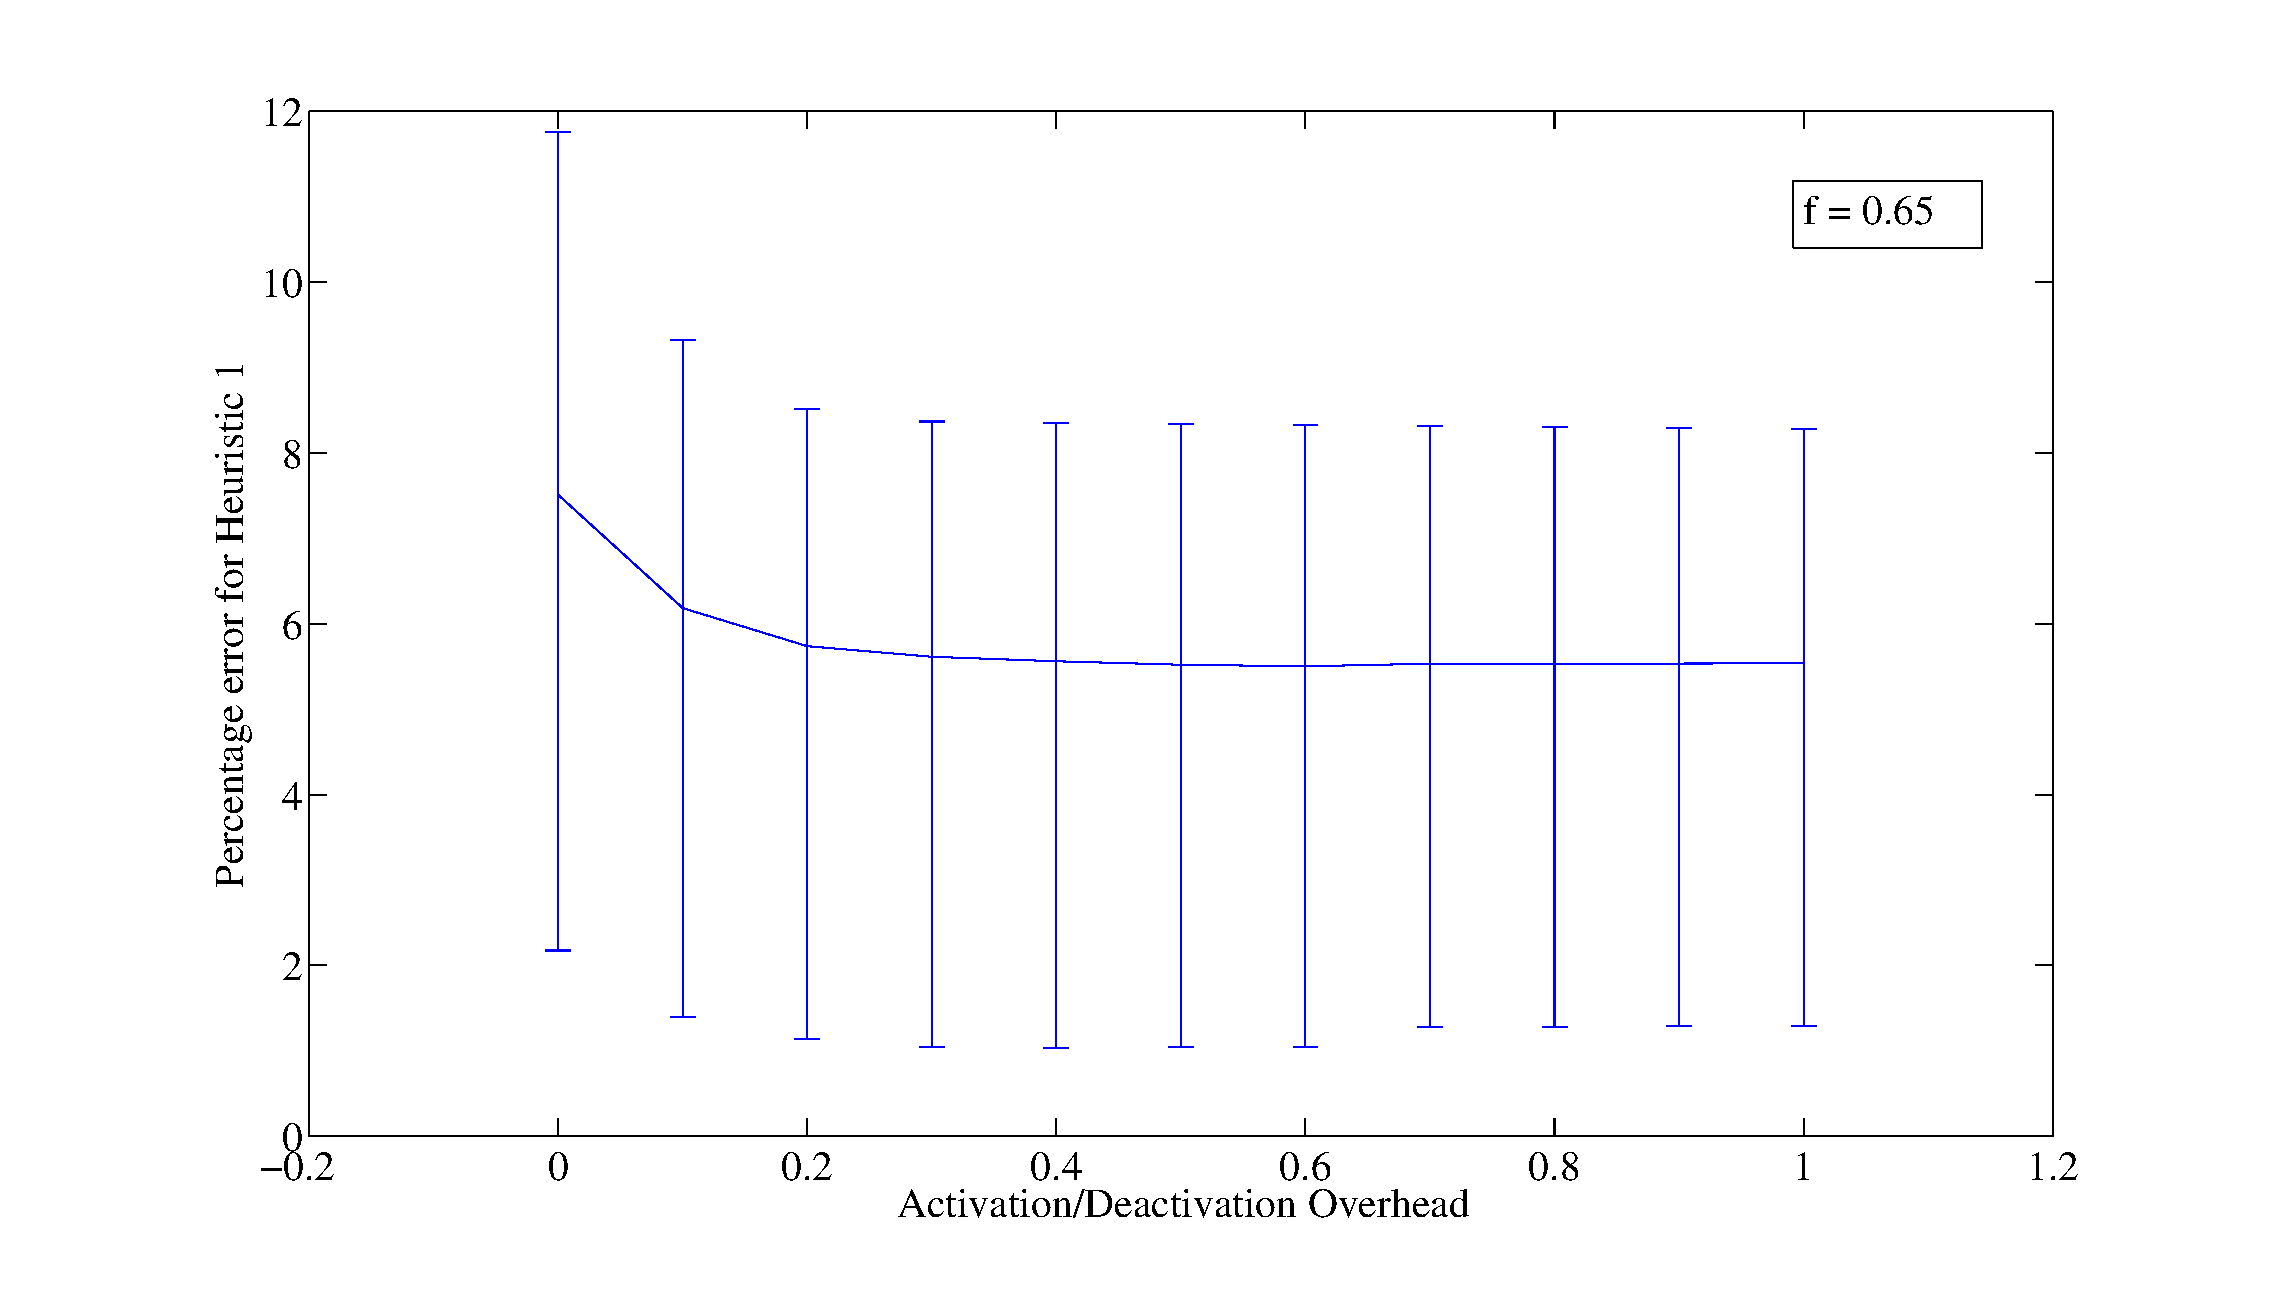
\includegraphics[width=1\linewidth]{../Matlab/rb-heur1error.eps}
\caption{Heuristic 1 performance}
\label{fig:heur1perf}
\end{figure}